\documentclass{uofsthesis-cs}

% Documentation for the uofsthesis-cs class is given in uofsthesis-cs.dvi
% 
% It is recommended that you read the CGSR thesis preparation
% guidelines before proceeding.
% They can be found at http://www.usask.ca/cgsr/thesis/index.htm

%%%%%%%%%%%%%%%%%%%%%%%%%%%%%%%%%%%%%%%%%%%%%%%%%%%%%%%%%%%%%%%%%%%%%%%%%%%%%%
% FRONTMATTER - In this section, specify information to be used to
% typeset the thesis frontmatter.
  \usepackage{graphicx} 
%%%%%%%%%%%%%%%%%%%%%%%%%%%%%%%%%%%%%%%%%%%%%%%%%%%%%%%%%%%%%%%%%%%%%%%%%%%%%%

% THESIS TITLE
% Specify the title. Set the capitalization how you want it.
\title{SynVisio: A Multiscale Tool for Visualizing Genomic Conservation}

% AUTHOR'S NAME
% Your name goes here.
\author{Venkat Kiran Bandi}

% DEGREE SOUGHT.  
% Use \MSc or \PhD here
\degree{\MSc}         

% THESIS DEFENCE DATE
% Should be month/year, e.g. July 2004
\defencedate{December/2019}


% NAME OF ACADEMIC UNIT
%
% The following two commands allow you to specify the academic unit you belong to.
% This will appear on the title page as
% ``<academic unit> of <department>''.
% So if you are in the division of biomedical engineering you would need to do:
% \department{Biomedical Engineering}
% \academicunit{Division}
%
% The default is ``Department of Computer Science'' if these commands
% are not given.
%
% If you are in a discipline other than Computer Science, uncomment the following line and
% specify your discipline/department.  Default is 'Computer Science'.
% \department{If not Computer Science, put the name of your department here}

% If you are not in a department, but say, a division, uncomment the following line.
% \academicunit{Put the type of academic unit you belong to here, e.g. Division, College}


% PERMISSION TO USE ADDRESS
%
% If you are not in Comptuer Science you will want to change the
% address on the Permission to Use page.  This is done using the
% \ptuaddress{}.  Example:
%
% \ptuaddress{Head of the Department of Computer Science\\
% 176 Thorvaldson Building\\
% 110 Science Place\\
% University of Saskatchewan\\
% Saskatoon, Saskatchewan\\
% Canada\\
% S7N 5C9
% }

% ABSTRACT
\abstract{
Due to rapid advancements in sequencing technologies high resolution genomic data is readily available for a wide range of species. However, analysing this huge volume of data is still a tedious task. While most genomic analysis tasks can be automated some still require human judgement and manual interpretation. One example of such a task is synteny analysis. Synteny is a key tool in comparative genomic research - it is the study of homologous regions within chromosomes of the same or different species. Visualizing synteny can help researchers in understanding the \textbf{location, size and orientation} of shared sequences among genomes of interest. However, the current tools which exist for synteny analysis are stand-alone programs or command line tools that are difficult to use and that offer very little interactivity. In this paper we provide a decentralized web-based environment for browsing syntenic blocks with multiple visual representations in the form of linear charts, hive charts and dot plots. Our tool also makes it easy to save and revisit graphs so that researchers can iteratively refine their plots and compare them with previous revisions for changes. We present SynVisio, a multiscale synteny analysis tool that provides multiple visualizations of genome collinearity for easy exploration across different scales from the whole genome level to the gene block level.
}

% THESIS ACKNOWLEDGEMENTS -- This can be free-form.
\acknowledgements{
Acknowledgements go here.  Typically you would at least thank your supervisor.
}

% THESIS DEDICATION -- Also free-form.  If you don't want a dedication, comment out the following
% line.
\dedication{This is the thesis dedication (optional)}

% LIST OF ABBREVIATIONS - Sample  
% If you don't want a list of abbreviations, comment the following 4 lines.
\loa{\abbrev{SCUBA}{Self Contained Underwater Breathing Apparatus}
\abbrev{LOF}{List of Figures}
\abbrev{LOT}{List of Tables}
}

%%%%%%%%%%%%%%%%%%%%%%%%%%%%%%%%%%%%%%%%%%%%%%%%%%%%%%%%%%%%%%%%
% END OF FRONTMATTER SECTION
%%%%%%%%%%%%%%%%%%%%%%%%%%%%%%%%%%%%%%%%%%%%%%%%%%%%%%%%%%%%%%%%

\begin{document}

% Typeset the title page
\maketitle

% Typeset the frontmatter.  
\frontmatter

%%%%%%%%%%%%%%%%%%%%%%%%%%%%%%%%%%%%%%%%%%%%%%%%%%%%%%%%%%%%%%%%
% FIRST CHAPTER OF THESIS BEGINS HERE
%%%%%%%%%%%%%%%%%%%%%%%%%%%%%%%%%%%%%%%%%%%%%%%%%%%%%%%%%%%%%%%%
\chapter{Introduction}

With the emergence of new sequencing systems genomic data is being generated at an unprecedented rate.Almost two decades back \textbf{The Human Genome Project} took 13 years and over 3 billion dollars to sequence the entire human genome whereas the same information can be sequenced today in under an hour for 1000 dollars.This rapid improvement in sequencing genomic data has improved the availability of high resolution genomics data and has helped researchers in answering a wide range of biological questions.


% reference to https://www.genome.gov/human-genome-project/Completion-FAQ


An important field in biological research where genomic data is extensively used is comparative genomics.It involves comparing genomic information between different species to understand their similarity.A genome of an organism consists of its complete set of DNA in the form of a series of genes where every gene is a sequence that is responsible for one or more traits in that organism.Comparing genomic sequences between two different organisms can help researchers in understating their evolutionary relationship as similar sequences can often mean that the genes have the same function.Such similar sequences are referred to as homologous sequences and they indicate shared ancestry.As organism evolve overtime and diversify into different species they retain parts of their DNA from their common ancestor.The study of these conserved homologous regions is called \textbf{Synteny}. 

While a huge part of comparing large scale genomic sequences is purely computational and thus can be automated human judgement is still vital in syteny analysis.Visual data exploration for example can help researchers in easily identifying similarities among large scale genomes as humans are intuitively good at picking out patterns in pictures and visuals.Synteny visualization commonly involves visualizing genomes at the whole genome level or the individual chromosome level and representing similar genes either by connected links or similar colored regions.Syntenic data analysis can often be an iterative process where researchers visualize computational results multiple times under various parameters such as the size and orientation of similar genes based on a given biological hypothesis.

The choice of visual encoding in the representation of syntenic relationship is dependant on the kind of analysis that is being done by the researchers.Certain graphical representations like dot plots where every conserved gene is represented as a point on a two dimensional matrix, are useful in analyzing extremely large genomes in a single representation as shown in Figure \ref{fig:ch_1_dot_plot} while other representations like linear horizontal plots where syntenic links are represented as coloured ribbons connecting similar regions are useful in performing a more in depth analysis as the conserved regions are more visually prominent.Additionally Circos plots which use a circular ideogram layout as shown in Figure \ref{fig:ch_1_circos_plot} are also used by researchers commonly in publications as they can be aesthetically pleasing.

With such varied graphical representations, arriving at the right form of visualization can be difficult and any system that offers only a single kind of visual encoding can become limited in its usability for a wide range of biological scenarios.Apart from looking at synteny in multiple representations researchers are also often interested in  investigate specific conserved regions further and thus needing the visualization system to be adaptive based on the genomic scale of interest.Thus visualizations systems need to go beyond acting as basic chart generating systems and instead offer a rich interactive experience where researchers can explore sequences from the whole genome level all the way down to the individual gene level in multiple graphical representations.

A key part of every visualization system is the data that drives it and genomic data owing to its large volume, is being increasingly managed and distribution through several online databases like NCBI and genBank.This rapid dissemination of data across the internet has created a need for visualization systems to be easily available across the web so researchers can collaborate and share their work.


\begin{figure}
\centering
\begin{minipage}{.5\textwidth}
  \centering
  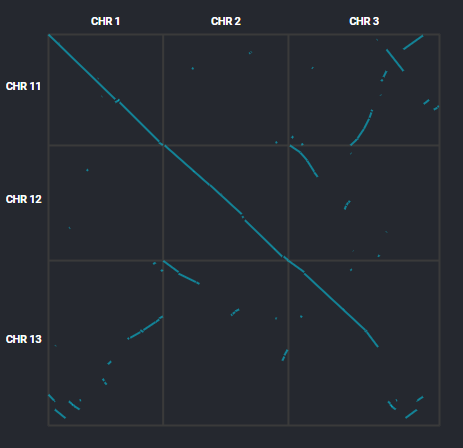
\includegraphics[width=.75\linewidth]{images/ch_1_dot_plot.PNG}
  \captionof{figure}{Dot plot}
  \label{fig:ch_1_dot_plot}
\end{minipage}%
\begin{minipage}{.5\textwidth}
  \centering
  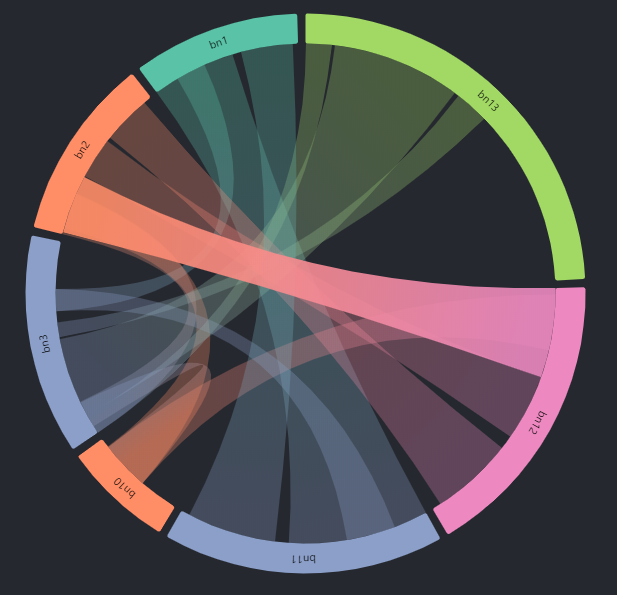
\includegraphics[width=.75\linewidth]{images/ch_1_circos_plot.PNG}
  \captionof{figure}{Circos Plot}
  \label{fig:ch_1_circos_plot}
\end{minipage}
\end{figure}


\section{Problem and Motivation}

The problem addressed in this thesis is: \textit{existing synteny tools are limited in their accessibility, offer little or no interactive experience and aren't integrated with the existing synteny detection tools to offer a seamless experience.}

Owing to the complexity involved in generating visualizations of large scale genomes, synteny visualization tools are largely command line based or stand alone programs limited to working in specific operating systems.This combined with the steep learning curve in using these systems means that a large set of these tools aren't accessible to the wider science community.Of the few online visualizations systems that exist, most act as simple chart generation systems instead of offering researchers chance to explore their datasets.This has largely pushed visualization into the report generation stage instead of the  iterative hypothesis testing phase of the research cycle.

Understanding genomic conservation is crucial for researchers as it has applications in a wide variety of scenarios such as predicting whole genome duplication events,sequencing extremely large genome sequences like wheat and classifying the proximity of different species in their evolutionary history.
While visualization systems are important as report generating tools that can create publication ready charts they need to move to earlier stages of the stages of the research cycle to accelerate the process of hypothesis testing.
Researchers should have the ability to interact with their datasets and change parameters in real time to see their results in easily understandable visual,
which in turn can let researchers explore a wide range of biological scenarios in a short span of time.
% refer vgsc

\section{Solution}

\begin{figure}
  \centering
  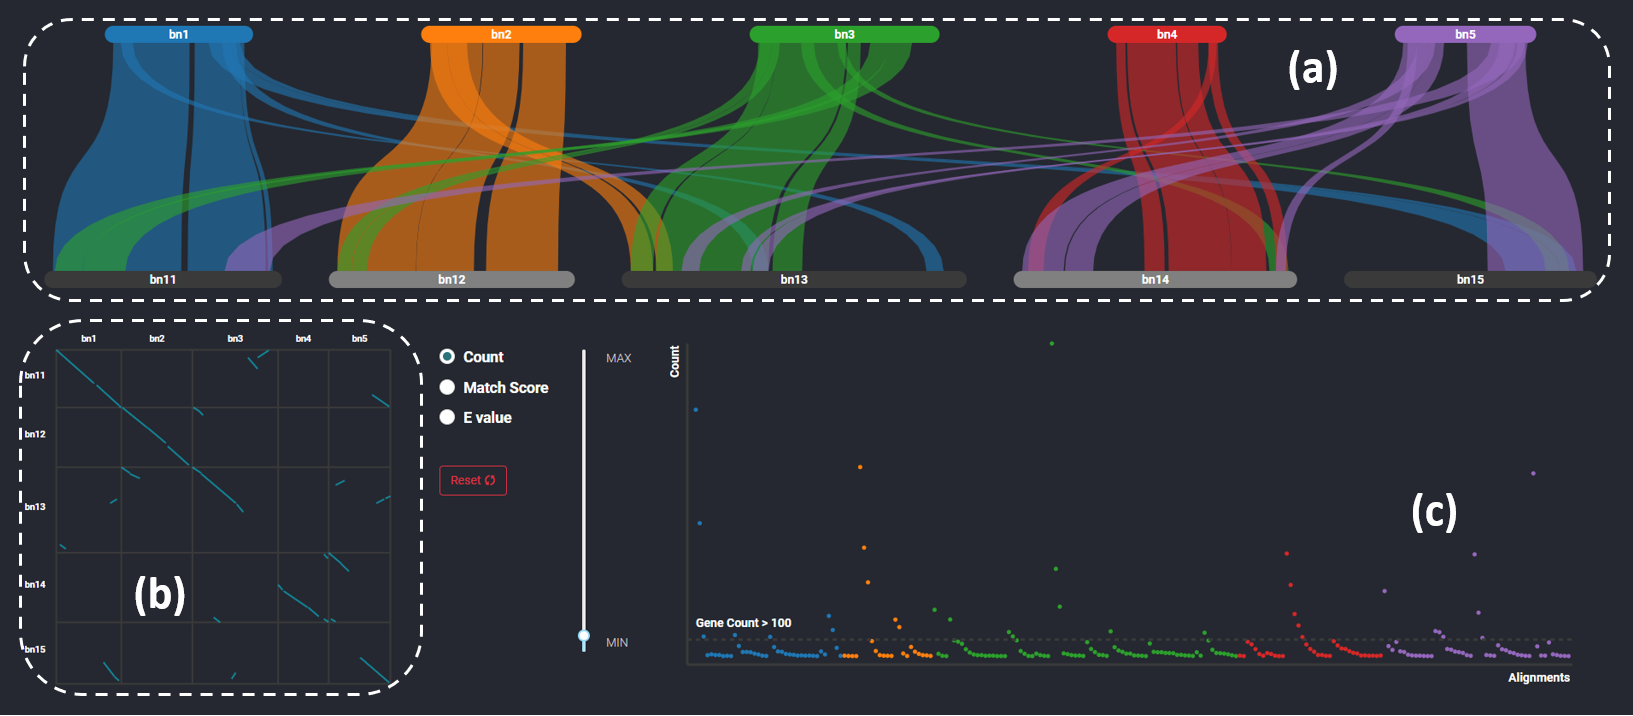
\includegraphics[width=.75\linewidth]{images/ch_1_dashboard.PNG}
  \captionof{figure}{Syteny Dashboard visualizing genome collinearity in Bn(Brassica Napus) with the following components: \textbf{a)} Linear Horizontal Plot with connected ribbons representing collinear gene blocks. \textbf{b)}Dot plot where every collinear gene is represented by a point and contiguous collinear blocks are shown as lines. \textbf{c)} Filter panel representing all the collinear blocks based on the count of their genes with ability to refine results using slider to the left.  }
  \label{fig:ch_1_dashboard}
\end{figure}

To address the lack of proper analysis tools in syteny research we developed \textbf{SynVisio} an online syteny visualization toolkit that can assist researchers in exploring genomic conservation.

\textbf{SynVisio} can directly work with results of existing syteny detecting tools like MCScanX and DAGChainer and can visualize conservation in multiple representations.It works in two modes,the basic synteny analysis mode lets users compare chromosomes in the same genome or between two genomes and the information is visualized as Horizontal linear plots,Dot plots or both as shown in Figure \ref{fig:ch_1_dashboard}.For visualizing synteny across several genomes simultaneously \textbf{SynVisio} offers a Multi-level analysis mode where synteny is visualized in stacked horizontal plots or Hive plots.\textbf{SynVisio} offers a rich interactive experience by letting users switch graphs in real time and explore data from genome level all the way down to the individual gene level.Users can do this by simply clicking on any two chromosomes when looking at a visualization in the genome level and then further step down from the individual chromosome level by clicking on a particular gene block to look at its constituent  genes and their orientation. Additionally users also have the ability to annotate their charts with additional genomic data in the form of tracks above the genomes or chromosomes which can be visualized as heat-maps,histograms or scatter-plots.



By default \textbf{SynVisio} lets users select the chromosomes that they wish to explore and then visualizes the conserved gene blocks in a dashboard that shows both the Horizontal linear plot and a Dot plot along with a filter panel where users can refine the results using a slider based on the level of similarity and the number of contiguous genes in a conserved block.
As users explore the synteny results \textbf{SynVisio} offers them the ability to records their interactions as snapshots which can be revisited or reset giving the ability to explore multiple scenarios and switch between them.The system also indexes all the conserved genes in the browser thus letting users quickly lookup genes by their gene IDs to see which conserved blocks they belong to.Finally \textbf{SynVisio} offers users the ability to download all the charts in transform and scale invariant vector graphics for research publication.

\section{Steps to the Solution} 
There were several steps involved in designing a system that could let researchers explore syteny through an easily accessible web based based tool.

\begin{itemize}
    
    \item \textbf{Formulate Design Requirements} -
    To characterize the needs from the biological research community we primarily met with three groups of researchers studying genomic conservation through a series of structured interviews to collect their requirements.The first group we met was interested in exploring syteny in wheat while the other two groups were involved in studying Canola and Pulse crops respectively.All three groups were unanimous in the verdict that syteny is a critical issue to study for understanding genomic evolution and that existing tools don't meet their needs.Based on the feedback from the genomic research community all requirements can be broadly classified into either \textbf{functional} or \textbf{non functional} requirements.Functional requirements primarily include understanding the size,location and orientation of conserved sequences along with having the ability to filter sequences based on their similarity while non functional requirements include features like the ability to download images or snapshot explorational points to revisit.
    
    \item \textbf{Research Existing Alternatives} - 
    Since synteny analysis is a combination of syteny detection followed by downstream analysis using visualization systems we looked at tools that operate in both these domains.We looked at several state of the art syteny detection packages like MCScanX, DAGChainer, Cyntenator and i-ADHoRe and also tested the visual outputs of some that had their own downstream analysis tools.We focused our research on MCScanX and DAGChainer out of the other alternatives as they were the most popular and frequently used tools by the researchers we interviewed and had easier and more efficient output data formats.We followed this by looking at the tools that worked  in the second stage of the analysis pipeline by providing visualizations like SynChro, GSV,Mizbee,VGSC and Circos.Of these we found that most served as simple graphic generating systems instead of offering a platform for detailed analysis except for MizBee which was however limited by its accessibility and limited variety in charts.We finally refined our initial requirements based on the characterization of the problem domain by some of these earlier tools like MizBee.

    \item \textbf{Choice of Visual Encoding and System Architecture} - 
    To implement our solution we decided on a web based single page tool that would work as a part of the existing analysis pipeline by working directly on the results of existing syteny detection tools.We adopted a thick-client architecture model as opposed to a thin client model where visualizations are generated on the server as this would let researchers directly upload their synteny analysis files and see the resulting images in real time without their sensitive data being sent to a remote server.To visually represent genomic conservation we used linear connections (horizontal plots)and points(dot plots) and then encoded additional information about the size and orientation of the gene blocks through a combination of colour and shape.
    To render the visualizations we used both canvas and simple vector graphics and tested both and found that the latter while being more resource intensive offered a better visual experience across multiple device sizes and resolution as it was transform and scale variant.So our system was designed to initially renders all charts as simple vector graphics but dynamically switch to canvas rendering for large scale genomes.The final application was developed through several design iterations as the system was used by our expert user group and several additional features not in our original requirements like support for additional tracks and the ability to download images were added based on their feedback. 

\end{itemize}

\section{Evaluation}
\section{Thesis Outline}

\chapter{Related Work}
%%%%%%%%%%%%%%%%%%%%%%%%%%%%%%%%%%%%%%%%%%%%%%%%%%%%%%%%%%%%%%%
% SUBSEQUENT CHAPTERS (or \input's)  GO HERE
%%%%%%%%%%%%%%%%%%%%%%%%%%%%%%%%%%%%%%%%%%%%%%%%%%%%%%%%%%%%%%%

%%%%%%%%%%%%%%%%%%%%%%%%%%%%%%%%%%%%%%%%%%%%%%%%%%%%%%%%%%%%%%%%
% The Bibliograpy should go here. BEFORE appendices!
%%%%%%%%%%%%%%%%%%%%%%%%%%%%%%%%%%%%%%%%%%%%%%%%%%%%%%%%%%%%%%%%


% Typeset the Bibliography.  The bibliography style used is "plain".
% Optionally, you can specify the bibliography style to use:
% \uofsbibliography[stylename]{yourbibfile}

\uofsbibliography{880Paper}

% If you are not using bibtex, comment the line above and uncomment
% the line below.  
%Follow the line below with a thebibliography environmentand bibitems.  
% Note: use of bibtex is usually the preferred method.

%\uofsbibliographynobibtex


%%%%%%%%%%%%%%%%%%%%%%%%%%%%%%%%%%%%%%%%%%%%%%%%%%%%%%%%%%%%%%%%%%%%%%%%%
% APPENDICES
%
% Any chapters appearing after the \appendix command get numbered with
% capital letters starting with appendix 'A'.
% New chapters from here on will be called 'Appendix A', 'Appendix B'
% as opposed to 'Chapter 1', 'Chapter 2', etc.
%%%%%%%%%%%%%%%%%%%%%%%%%%%%%%%%%%%%%%%%%%%%%%%%%%%%%%%%%%%%%%%%%%%%%%%%%%

% Activate thesis appendix mode.
\uofsappendix

% Put appendix chapters in the appendices environment so that they appear correcty
% in the table of contents.  You can use \input's here as well.
\begin{appendices}

\chapter{Sample Appendix}

Stuff for this appendix goes here.

\chapter{Another Sample Appendix}

Stuff for this appendix goes here.

\end{appendices}

\end{document}
